\begin{figure}[h] 
\centering 
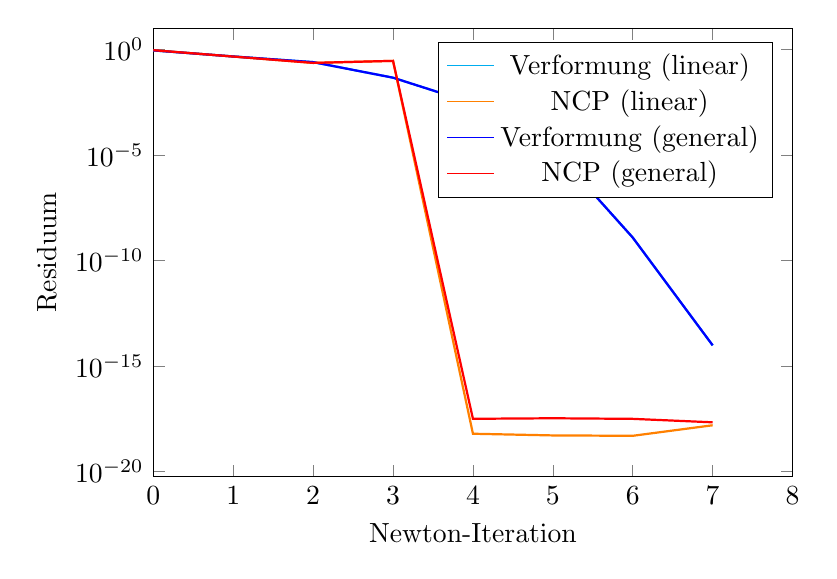
\begin{tikzpicture}[every plot/.append style={thick}] 
\begin{axis}[ 
label style={font=\normalsize}, 
xlabel={Newton-Iteration}, 
ylabel={Residuum}, 
xmin=0, xmax=8, 
ymode=log, 
ymin=0, ymax=10, 
width=0.8\textwidth, 
height=0.6\textwidth, 
legend pos=north east, 
legend style={cells={align=left}}, 
grid style=dashed, 
] 
\addplot[ 
color=cyan, 
] 
coordinates { 
(0, 8.90e-01)(1, 4.60e-01)(2, 2.48e-01)(3, 4.55e-02)(4, 2.80e-03)(5, 2.04e-05)(6, 1.22e-09)(7, 9.56e-15)}; 
\addlegendentry{Verformung (linear)} 
\addplot[ 
color=orange, 
] 
coordinates { 
(0, 9.12e-01)(1, 4.56e-01)(2, 2.28e-01)(3, 2.85e-01)(4, 6.27e-19)(5, 5.22e-19)(6, 5.01e-19)(7, 1.58e-18)}; 
\addlegendentry{NCP (linear)} 
\addplot[ 
color=blue, 
] 
coordinates { 
(0, 8.90e-01)(1, 4.60e-01)(2, 2.48e-01)(3, 4.55e-02)(4, 2.80e-03)(5, 2.04e-05)(6, 1.22e-09)(7, 9.66e-15)}; 
\addlegendentry{Verformung (general)} 
\addplot[ 
color=red, 
] 
coordinates { 
(0, 9.12e-01)(1, 4.56e-01)(2, 2.28e-01)(3, 2.85e-01)(4, 3.20e-18)(5, 3.39e-18)(6, 3.18e-18)(7, 2.18e-18)}; 
\addlegendentry{NCP (general)} 
\end{axis} 
\end{tikzpicture} 
\caption{Residuen des Stoffgesetzes 'St.Venant' mit Hinderniss 'Spitze' und 578 Freiheitsgraden für die Verschiebung.} 
\label{fiq:St.Venant_Spitze_level3} 
\end{figure} 
